\chapter{Quantum-Resistant Cryptography}\label{chap:quantum_resistant}

The demonstration in Chapter \ref{chap:quantum_impact} that quantum computers, particularly leveraging \gls{shors-algorithm}, can efficiently break currently deployed \gls{public-key-cryptography} systems like \gls{rsa} and \gls{ecc}, necessitates a fundamental shift towards cryptographic algorithms secure against both classical and quantum adversaries. This field is known as \gls{post-quantum-cryptography} (PQC) or quantum-resistant cryptography. PQC does not rely on quantum phenomena itself for security; rather, it employs classical cryptographic techniques based on mathematical problems believed to be computationally hard even for large-scale quantum computers \parencite{bernstein2017post}. This chapter introduces the primary families of PQC algorithms, discusses the ongoing standardization efforts, and touches upon key implementation considerations.

\section{Introduction to Post-Quantum Cryptography}\label{chap:pqc_overview}
Recognizing the threat posed by quantum computers, the cryptographic community has been actively researching and developing \gls{post-quantum-cryptography} (PQC)---algorithms designed to be secure against attacks from both classical and sufficiently powerful quantum computers \parencite{bernstein2017post}.

\section{Major Families of Post-Quantum Cryptography}\label{sec:pqc_categories_ch5}
Post-quantum algorithms are typically categorized into several main families based on the underlying mathematical problems they rely on for security. These problems are believed to be hard for both classical and quantum computers to solve efficiently. The primary families include:

\subsection{Lattice-Based Cryptography}\label{subsec:lattice_ch6}\label{subsec:lattice_ch5}
Among the diverse approaches to \gls{post-quantum-cryptography}, schemes based on mathematical lattices have emerged as particularly prominent and versatile. Their security is rooted in the presumed computational difficulty of solving certain geometric problems defined over these lattices, problems believed to remain hard even for quantum computers \parencite{bernstein2017post}.

\subsubsection{Understanding Lattices}
Imagine a regular, repeating pattern of points extending infinitely in multiple dimensions. This is the essence of a mathematical lattice. More formally, given a set of linearly independent vectors $\mathbf{v}_1, \mathbf{v}_2, \dots, \mathbf{v}_n$ in $n$-dimensional space (called the basis vectors), the lattice $L$ generated by this basis is the set of all possible points you can reach by taking integer linear combinations of these basis vectors:
\begin{equation*}
    L = \left\{ \sum_{i=1}^{n} a_i \mathbf{v}_i \mid a_i \in \mathbb{Z} \right\}
\end{equation*}
where $\mathbb{Z}$ represents the set of all integers (positive, negative, and zero). Think of a 2D lattice like an infinite sheet of graph paper, but where the grid lines might be skewed or stretched depending on the choice of basis vectors (as conceptually shown in Figure~\ref{fig:lattice_2d_basis}). The same basis vectors can generate the same infinite set of points, making finding the "best" basis a non-trivial task.

\begin{figure}[ht]
    \centering
    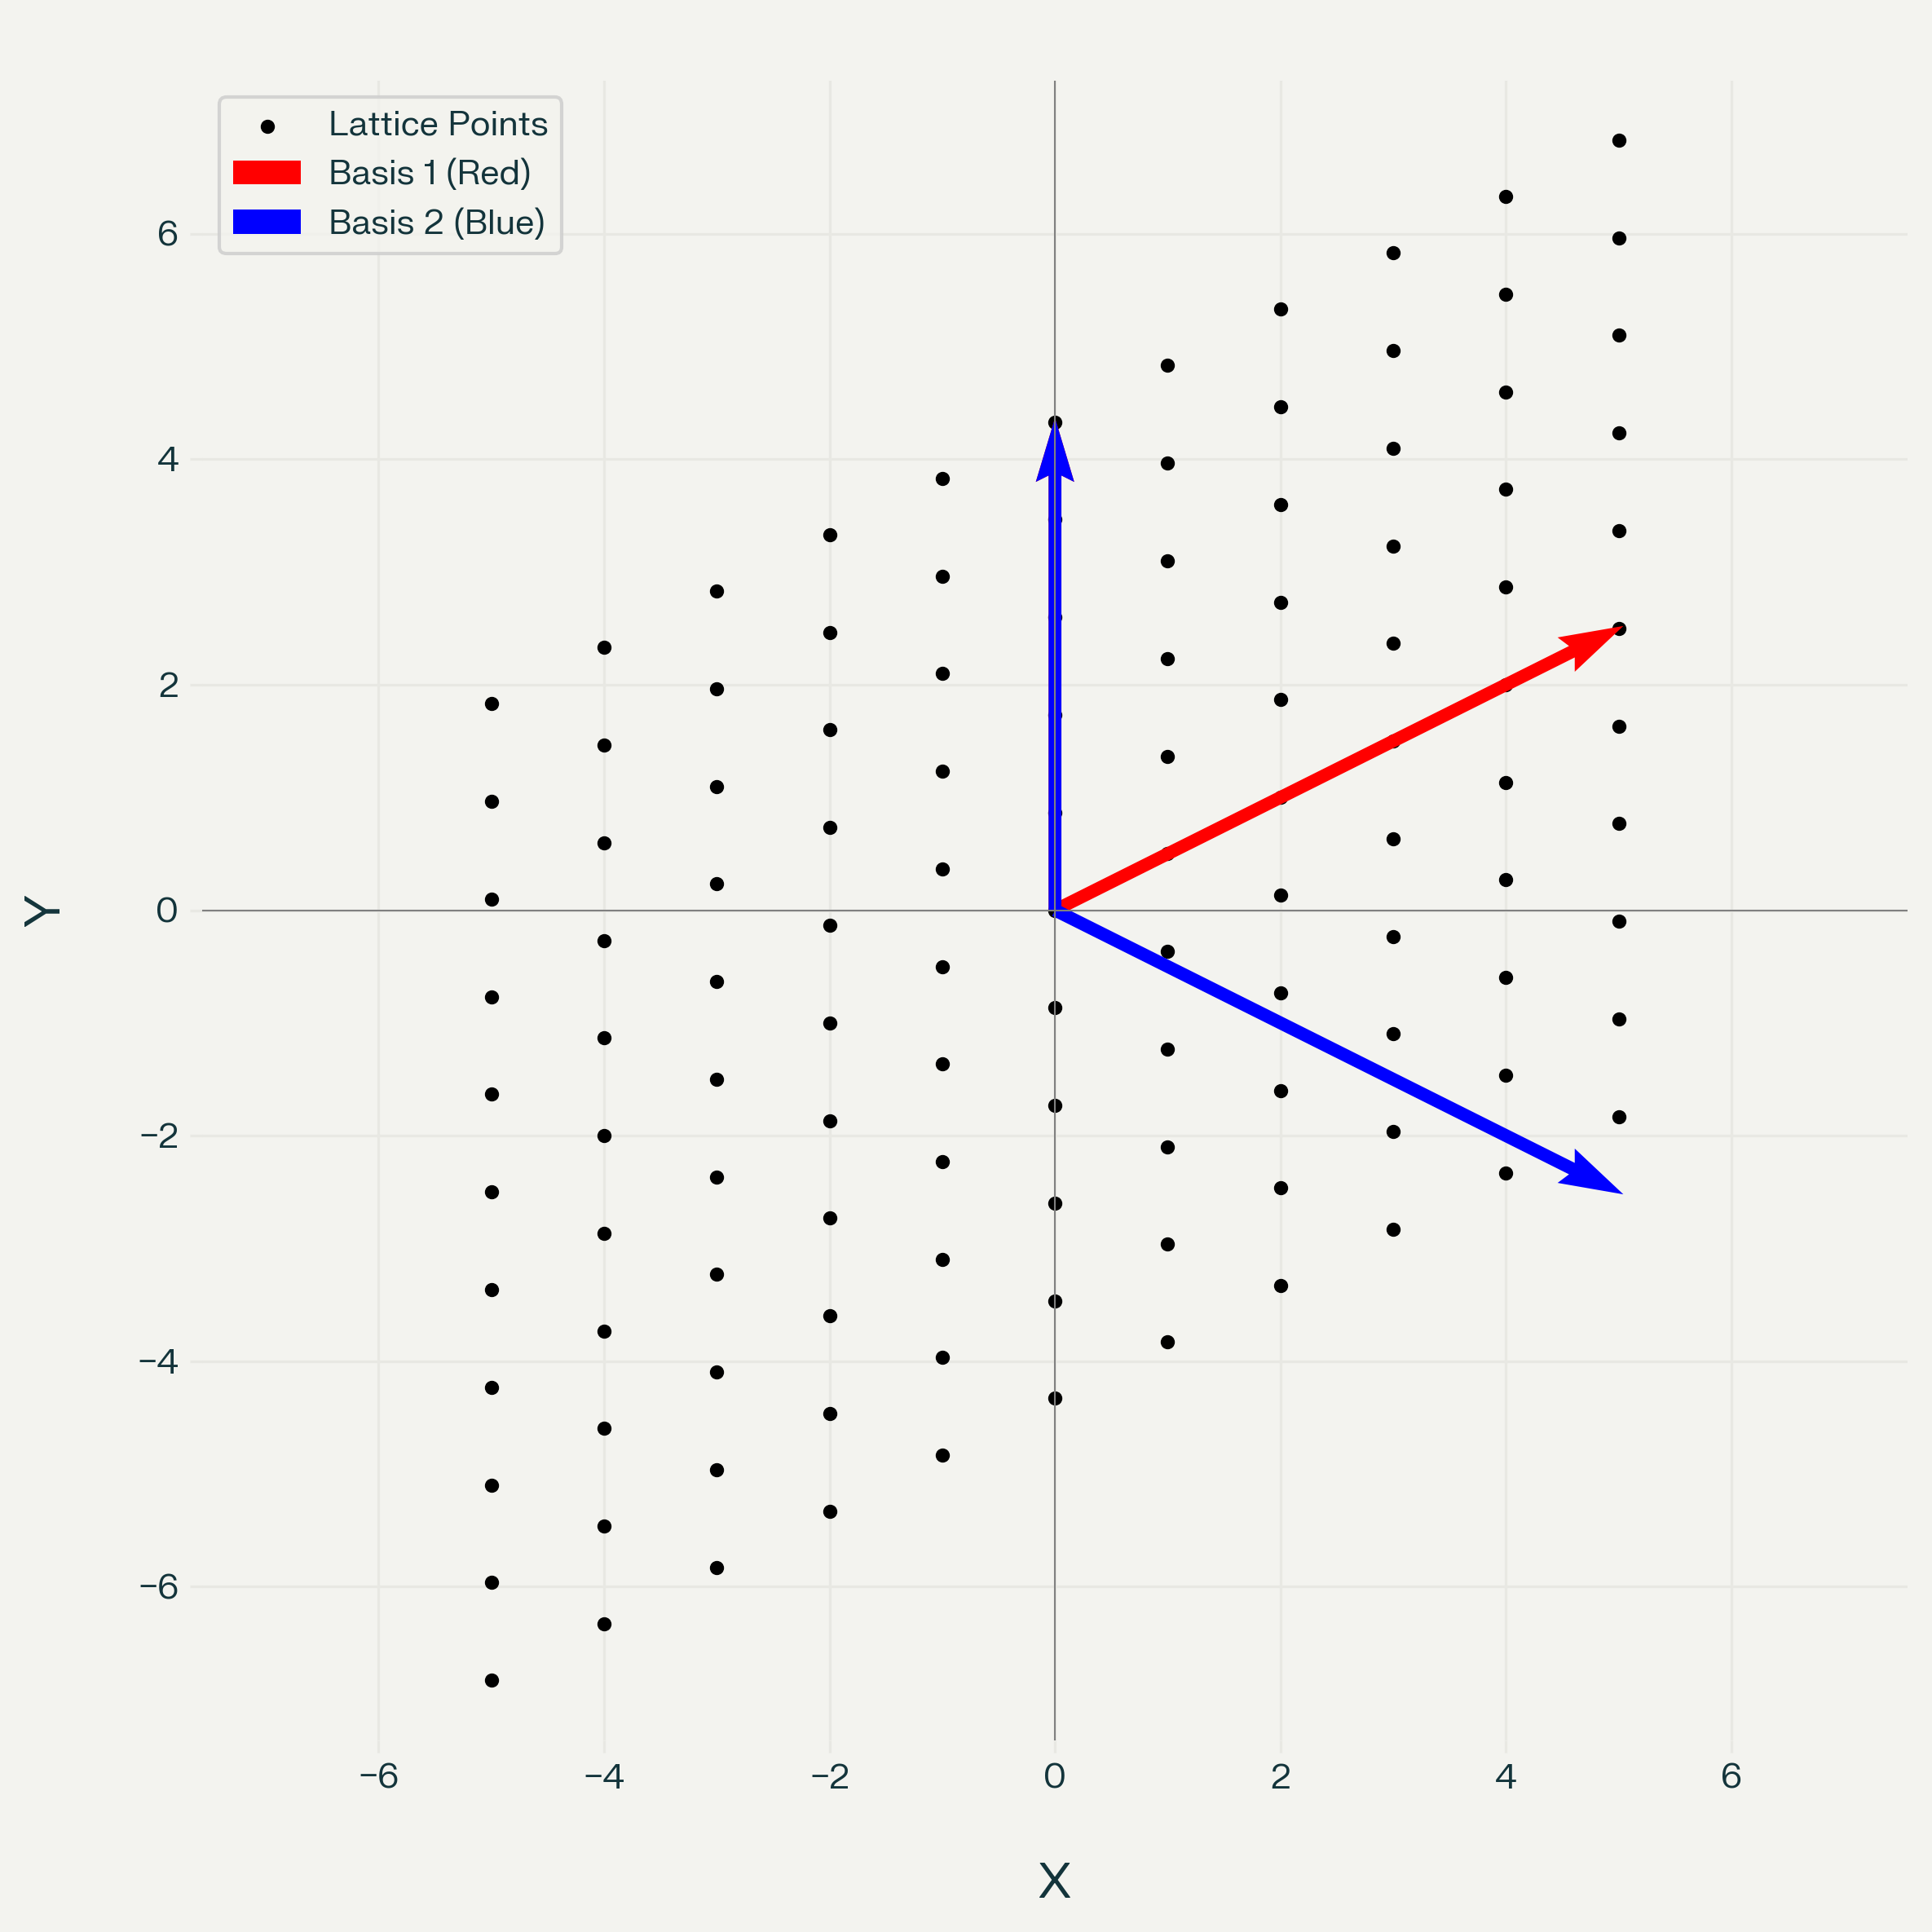
\includegraphics[width=0.6\textwidth]{src/images/06_Challenges_in_Transition/lattice_2d_fundament} % COMMENTED OUT - File missing
    \caption{A 2D lattice showing two different bases (red and blue vectors) that generate the same set of points.}
    \label{fig:lattice_2d_basis} % Added missing figure label
\end{figure}
\newpage

\subsubsection{Hard Problems on Lattices}
While lattices have a regular structure, certain geometric problems defined on them become computationally very hard, especially as the number of dimensions increases. The security of lattice-based cryptosystems typically relies on the difficulty of problems like:
\begin{itemize}
    \item \textbf{Shortest Vector Problem (SVP):} Finding the non-zero lattice point closest to the origin (the zero vector). While easy to visualize in 2D (see Figure~\ref{fig:lattice_svp_cvp}), finding this shortest vector becomes exponentially difficult in high dimensions for known classical and quantum algorithms.
    \item \textbf{Closest Vector Problem (CVP):} Given a target point $\mathbf{t}$ in the space (which may not be a lattice point itself), find the lattice point $\mathbf{p}$ that is closest to $\mathbf{t}$. Again, this is computationally hard in high dimensions (see Figure~\ref{fig:lattice_svp_cvp}).
\end{itemize}

\begin{figure}[ht]
    \centering
    % Replace TikZ with image
    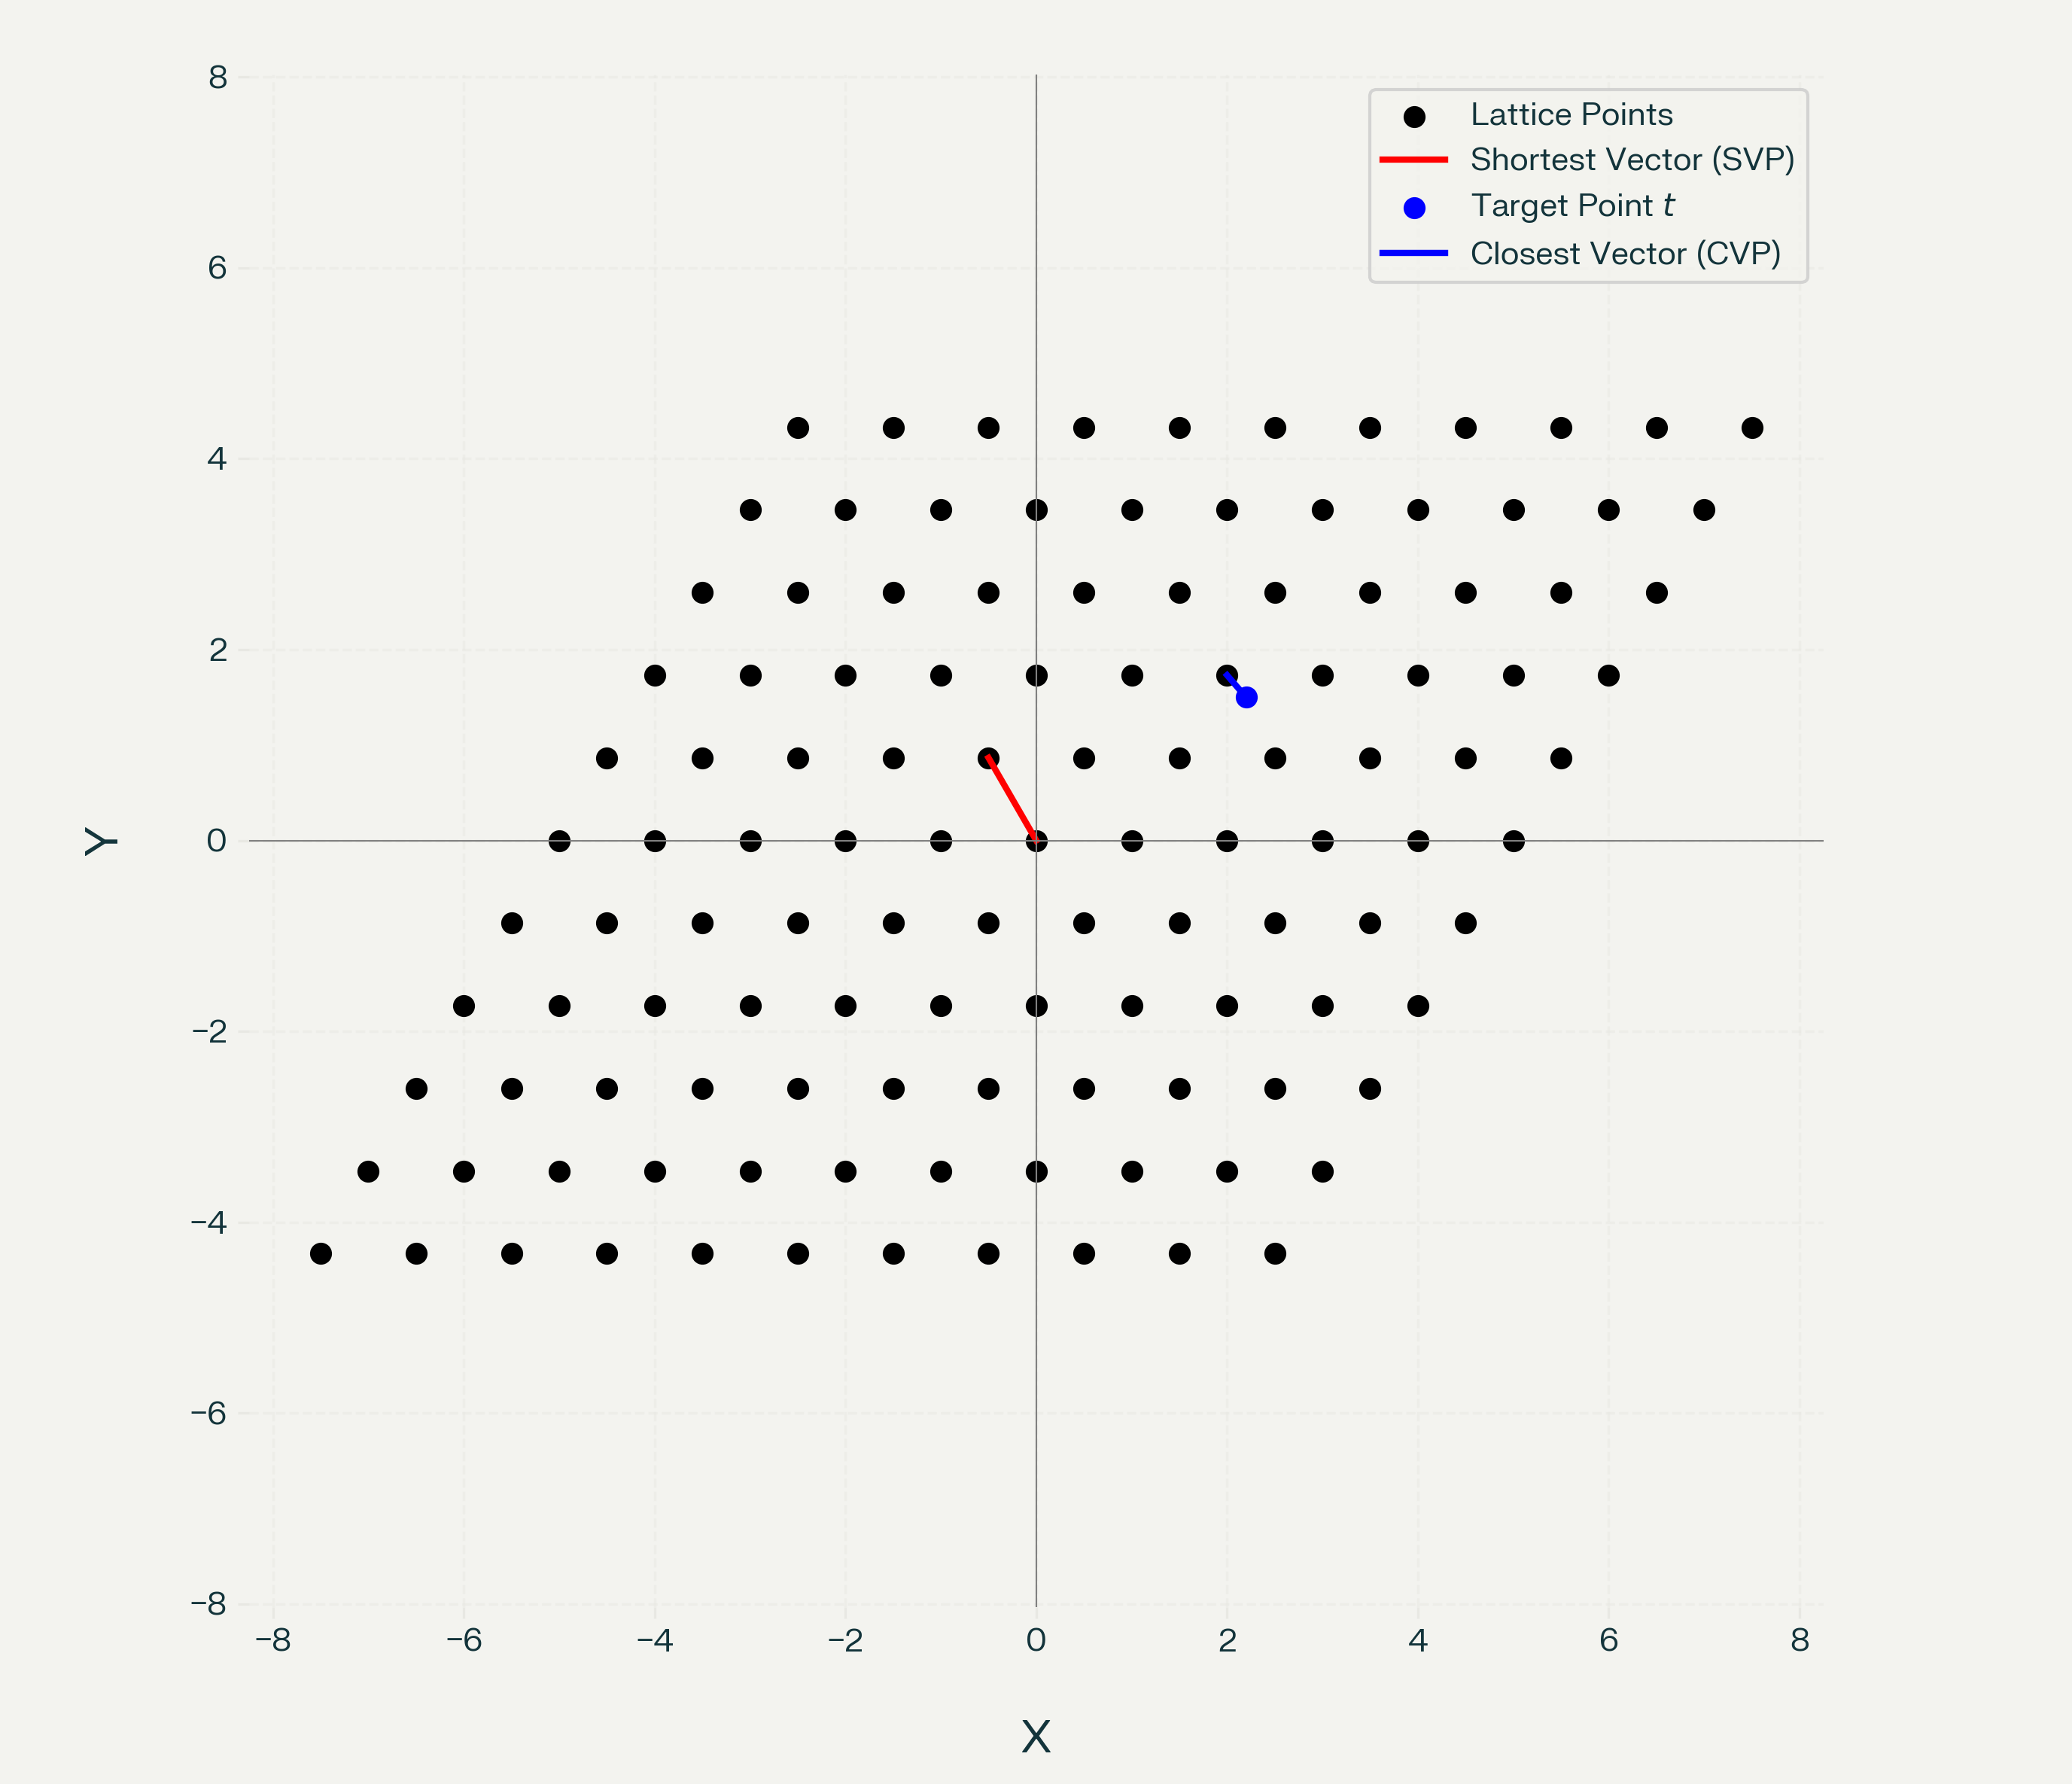
\includegraphics[width=0.7\textwidth]{src/images/06_Challenges_in_Transition/latticeproblem.png} % Corrected Path
    \caption{Illustration of Lattice Problems: Shortest Vector Problem (SVP - find shortest vector, red) and Closest Vector Problem (CVP - find lattice point nearest target $t$, blue).}
    \label{fig:lattice_svp_cvp} % Added missing figure label
\end{figure}

While SVP and CVP are fundamental, modern lattice cryptography often relies more directly on the \textbf{\Gls{lwe} (Learning With Errors)} problem, introduced by Oded Regev \parencite{peikert2016decade}. LWE provides a powerful framework for building cryptographic schemes.
\newpage

\subsubsection{The Learning With Errors (LWE) Problem}
Imagine trying to determine a secret set of numbers (a secret vector $\mathbf{s}$) when you are only given clues in the form of approximate linear equations. This is the core idea behind LWE. An adversary is given access to multiple samples $(\mathbf{a}_i, b_i)$. Each $\mathbf{a}_i$ is a known, randomly chosen vector, and $b_i$ is approximately equal to the inner product (dot product) of $\mathbf{a}_i$ and the secret $\mathbf{s}$, but with a small amount of random "noise" or "error" $e_i$ added:
\begin{equation*}
    b_i \approx \langle \mathbf{a}_i, \mathbf{s} \rangle + e_i \pmod{q}
\end{equation*}
Here, $q$ is a modulus (typically a prime number), and the error $e_i$ is drawn from a specific probability distribution, usually centered around zero with a small standard deviation (like a discrete Gaussian distribution). The challenge for the adversary is to recover the secret vector $\mathbf{s}$ using only the publicly known $\mathbf{a}_i$ vectors and the noisy results $b_i$.

% Suggestion for Figure fig:lwe_conceptual
\begin{figure}[h]
    \centering
     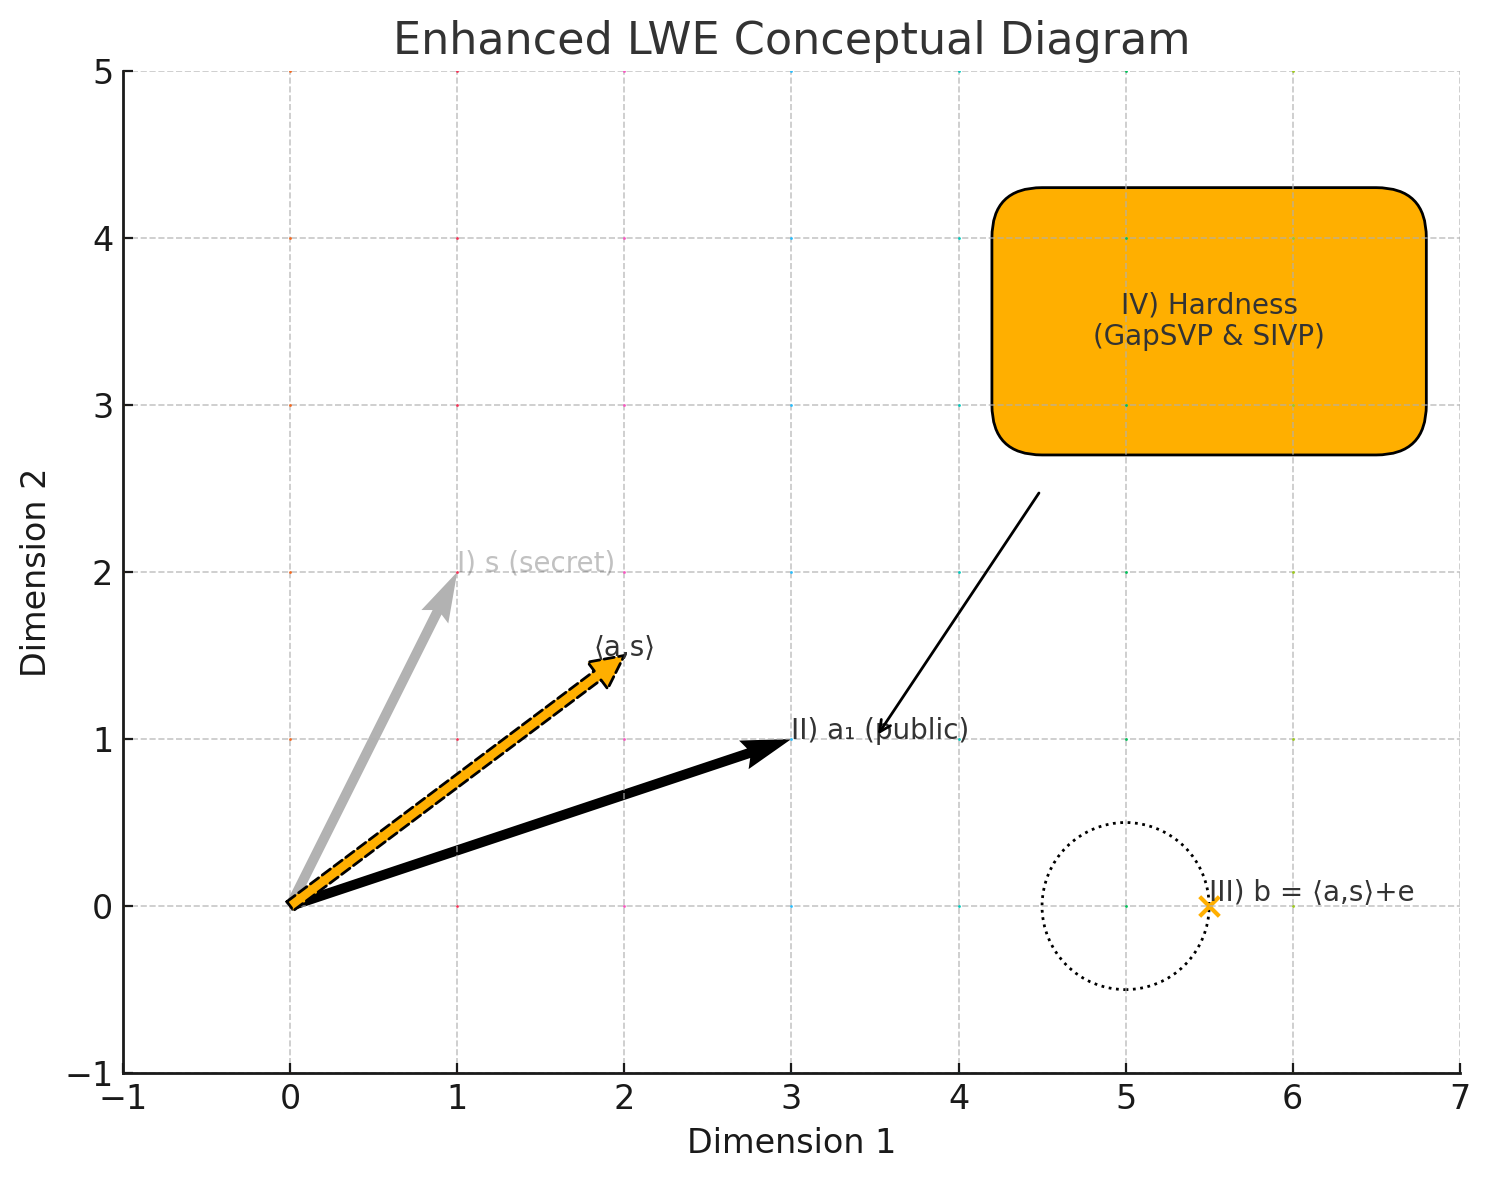
\includegraphics[width=0.8\textwidth]{src/images/06_Challenges_in_Transition/lwe} % Replace with actual diagram
    \caption{Conceptual illustration of the LWE problem: Recovering the secret $\mathbf{s}$ from public samples $(\mathbf{a}_i, b_i)$ where $b_i$ is the inner product $\langle \mathbf{a}_i, \mathbf{s} \rangle$ plus small noise $e_i$.}
    \label{fig:lwe_conceptual}
\end{figure}

Without the noise ($e_i = 0$), finding $\mathbf{s}$ would be a standard linear algebra problem, easily solvable classically. However, the addition of these small, random errors fundamentally changes the problem's nature, making it computationally difficult. It essentially hides the secret $\mathbf{s}$ within the uncertainty introduced by the noise. The security relies on the fact that distinguishing the distribution of $(\mathbf{a}_i, b_i)$ pairs from a distribution where $b_i$ is simply chosen uniformly at random is computationally hard.
\newpage

\subsubsection{Quantum Resistance of LWE}
The reason LWE is believed to be resistant to quantum computers stems from this reliance on noise and the lack of apparent exploitable structure. Unlike integer factorization or the discrete logarithm problem, which possess a periodic structure that \gls{shors-algorithm} can efficiently find using the \gls{qft}, the LWE problem does not seem to exhibit such periodicity \parencite{bernstein2017post}. The randomness introduced by the errors effectively masks any underlying algebraic structure that current quantum algorithms might target. While quantum computers might offer some speedup for lattice problems (e.g., using Grover's algorithm for search aspects), they do not provide the exponential advantage seen with Shor's algorithm against classical public-key systems. Therefore, LWE and related lattice problems form a strong foundation for building PQC schemes.

\subsubsection{Efficiency Variants: Ring-LWE and Module-LWE}
While standard LWE provides strong security guarantees, its practical implementations can lead to relatively large keys and slower computations. To improve efficiency, structured variants were developed:
\begin{itemize}
    \item \textbf{Ring-LWE:} Instead of working with generic vectors and matrices, Ring-LWE operates within the richer algebraic structure of polynomial rings. This allows mathematical operations to be performed much more efficiently using tools like the Number Theoretic Transform (NTT), significantly reducing key sizes and speeding up computations.
    \item \textbf{\Gls{module-lwe}:} This variant acts as an intermediate step between standard LWE and Ring-LWE. It works over mathematical structures called modules, which generalize the ring structure. Module-LWE aims to retain most of the efficiency benefits of Ring-LWE while potentially offering security guarantees closer to the more general (and arguably more conservative) standard LWE problem.
\end{itemize}
Many leading PQC candidates, including those selected by NIST, leverage the efficiency gains offered by Module-LWE \parencite{lattice_theory_2024}. However, the introduction of this extra algebraic structure necessitates ongoing security analysis to ensure no new vulnerabilities are inadvertently created.
\newpage

\subsubsection{Strengths and Weaknesses}
Lattice-based cryptography offers a compelling package for the post-quantum era. Its \textbf{strengths} include strong theoretical security foundations often linked to worst-case problem hardness, versatility in building different cryptographic tools like \glspl{kem} and signatures, and generally efficient performance compared to some other PQC families. The underlying LWE concept is also relatively accessible compared to the intricacies of elliptic curve mathematics.

However, it is not without its \textbf{weaknesses}. A primary concern is the size overhead: public keys, ciphertexts, and signatures are typically larger than their counterparts in traditional ECC systems, which can pose challenges for protocols sensitive to bandwidth or storage (like TLS or constrained IoT devices). Selecting appropriate parameters (dimensions, modulus, noise level) to ensure both security and efficiency is a complex task requiring specialized knowledge. Furthermore, like all cryptographic implementations, lattice-based schemes require careful engineering to prevent vulnerabilities arising from \glspl{side-channel-attack}. Finally, while the underlying mathematical problems are well-studied, their widespread cryptographic application is newer than RSA or ECC, meaning they have faced less long-term, real-world cryptanalytic scrutiny, although the intensive NIST evaluation process has significantly mitigated this concern.

\subsubsection{NIST Standardized Examples}
The practical potential of lattice-based cryptography is underscored by its strong representation in the NIST PQC standardization outcome:
\begin{itemize}
    \item \textbf{CRYSTALS-Kyber:} Chosen as the primary standard for \glspl{kem}, Kyber leverages Module-LWE to provide a well-rounded balance of security, operational speed, and key/ciphertext sizes suitable for general-purpose key exchange. Kyber's design specifically targets efficiency and ease of implementation while maintaining robust security against known classical and quantum attacks. Its operations involve polynomial arithmetic in a ring modulo $q$, combined with techniques to generate shared secrets that are computationally indistinguishable from random values for an adversary without the private key. The security levels defined by NIST (Levels 1, 3, 5) correspond to varying parameter sets, offering different trade-offs between security margin and performance overhead \parencite{nist_pqc_fips_205}. The selection of Kyber reflects confidence in the underlying Module-LWE problem and its suitability for widespread deployment in protocols like TLS.
    \item \textbf{CRYSTALS-Dilithium:} Selected as a primary standard for digital signatures, Dilithium is also based on Module-LWE and offers efficient signing and verification, making it a strong general-purpose signature scheme.
    \item \textbf{Falcon:} Another primary signature standard, Falcon is built upon the NTRU lattice problem (closely related to Ring-LWE). Its main advantage is producing significantly smaller signatures than Dilithium, which is valuable in size-constrained scenarios. However, its implementation is more complex, notably requiring floating-point arithmetic during the signing process.
\end{itemize}
These standardized algorithms provide developers with concrete, rigorously analyzed options for implementing quantum-resistant key establishment and digital authentication.
\newpage

\subsection{Hash-Based Cryptography}\label{subsec:hash_ch6}
\Gls{hash-based-cryptography}, particularly for digital signatures, relies solely on the security properties of cryptographic hash functions (like SHA-2 or SHA-3, see Section \ref{sec:hash_functions_ch3_rev}). Since hash functions are generally believed to be more resistant to quantum attacks (only quadratically weakened by \gls{grovers-algorithm}), hash-based signatures offer strong security guarantees with minimal mathematical assumptions beyond the hash function's security \parencite{hash_based_advances_2024}.

Early hash-based signatures (e.g., Lamport signatures) were one-time signatures (OTS), meaning a key pair could only sign a single message securely. Modern schemes build upon these using Merkle trees to combine many OTS keys into a single public key that can sign multiple messages. There are two main types:
\begin{itemize}
    \item \textbf{Stateful Signatures (e.g., XMSS, LMS):} Offer smaller signatures and faster signing but require the signer to securely maintain state (e.g., tracking which OTS key was used last). Using the same OTS key twice breaks security completely.
    \item \textbf{Stateless Signatures (e.g., SPHINCS+):} Eliminate the need for state management, making them safer to deploy in practice. However, this comes at the cost of significantly larger signature sizes (often tens of kilobytes) and slower signing performance compared to stateful schemes or lattice-based signatures.
\end{itemize}
\Gls{nist-pqc} selected \textbf{SPHINCS+} as the standard for stateless hash-based signatures due to its strong security foundations and avoidance of state management risks.

\subsection{Code-Based Cryptography}\label{subsec:code_ch6}\label{subsec:code_ch5}
Code-based cryptography, pioneered by McEliece \parencite{mceliece1978public}, relies on the difficulty of decoding a general linear code, which is an \gls{np-hard} problem. The foundational scheme is the McEliece cryptosystem, proposed in 1978. In McEliece, the public key is a generator matrix $G'$ for a specific code family (e.g., binary Goppa codes) that possesses an efficient decoding algorithm. This matrix $G'$ is constructed by taking the original generator matrix $G$ of the chosen code and obfuscating it using a random non-singular matrix $S$ and a random permutation matrix $P$, such that $G' = SGP$. This transformation makes $G'$ appear as a generator matrix for a general random linear code, for which decoding is known to be an NP-hard problem \parencite{bernstein2008introduction}.

Encryption involves representing the message $m$ as a vector, computing the codeword $c = mG'$, and adding a random error vector $e$ of a specific weight $t$ (number of non-zero entries) to produce the ciphertext $y = c + e = mG' + e$. Decryption requires knowledge of the secret components $S$, $G$, and $P$. The recipient computes $y' = yP^{-1} = mSG + eP^{-1}$. Since $P$ is a permutation matrix, $e' = eP^{-1}$ has the same weight $t$. The recipient then uses the efficient decoding algorithm associated with the original code $G$ to decode $y'$ and recover $mS$. Finally, multiplying by $S^{-1}$ yields the original message $m$. The security relies on the intractability of decoding the publicly known code generated by $G'$ without knowledge of its hidden structure ($S$, $G$, $P$).

Code-based cryptography offers fast encryption and decryption but is primarily suited for encryption/\glspl{kem}. A major drawback has historically been very large public key sizes (hundreds of kilobytes to megabytes), although the ciphertext overhead is often small. Recent research and variants (like Niederreiter) aim to reduce key sizes. \Gls{nist-pqc} is standardizing \textbf{Classic McEliece} (using binary Goppa codes) as an additional \gls{kem}, valued for its long history (having withstood cryptanalysis since 1978), distinct security assumptions compared to lattices, and conservative parameter choices \parencite{code_based_2024, nist_pqc_status_report_ir8413}. Its inclusion in the NIST portfolio provides an alternative for applications where the large key size is acceptable and a diversity of cryptographic assumptions is desired.

\subsection{Multivariate Cryptography}\label{subsec:multivariate_ch6}
\Gls{multivariate-cryptography} bases its security on the difficulty of solving systems of multivariate polynomial equations over a finite field (the "MQ problem"). These schemes are generally better suited for digital signatures than encryption. They often feature very fast signature generation and verification and relatively small signatures. However, designing secure multivariate schemes has proven challenging; several proposals have been broken over the years. Furthermore, public keys can sometimes be large. NIST selected \textbf{Rainbow} as a finalist, but it was subsequently broken and is no longer being standardized \parencite{djelic2021nist}. Research continues in this area, but it currently holds fewer standardized candidates compared to lattice or hash-based approaches.

\section{NIST Standardization Process}

Recognizing the existential threat posed by quantum computers, the U.S. National Institute of Standards and Technology (NIST) initiated a public process in 2016 to solicit, evaluate, and standardize quantum-resistant cryptographic algorithms \parencite{nist_pqc}. This multi-year effort involved several rounds of submission, public analysis, and feedback from the global cryptographic community.

The goals were to select a portfolio of algorithms offering strong security against both classical and quantum attacks, good performance characteristics, and representing diverse mathematical approaches (to hedge against future cryptanalytic breakthroughs targeting a single family).

In July 2022, NIST announced its first set of selections for standardization \parencite{nist_pqc_status_report_ir8413}:
\begin{itemize}
    \item \textbf{For Public-Key Encryption / KEMs:} CRYSTALS-Kyber (primary standard).
    \item \textbf{For Digital Signatures:} CRYSTALS-Dilithium, Falcon, and SPHINCS+ (primary standards).
\end{itemize}
Additionally, NIST selected several algorithms for further evaluation in a fourth round, focusing on KEMs with different characteristics, including Classic McEliece, BIKE, and HQC. Final standards for the initial selections are expected soon, providing official specifications for implementation and deployment. This standardization process is crucial for enabling widespread adoption and interoperability of PQC solutions.
\newpage

\section{Implementation Considerations}

Deploying PQC algorithms involves practical considerations beyond theoretical security \parencite{pqc_optimization_2024}:
\begin{itemize}
    \item \textbf{Performance Trade-offs:} As discussed, different PQC families exhibit varying performance in terms of key generation speed, encryption/encapsulation speed, decryption/decapsulation speed, and the size of public keys, private keys, ciphertexts, and signatures. These trade-offs must be evaluated in the context of specific applications and protocols (e.g., TLS handshakes, code signing, disk encryption).
    \item \textbf{Implementation Security:} Like classical algorithms, PQC implementations are vulnerable to \glspl{side-channel-attack} (timing, power analysis, etc.) if not carefully implemented. Developing constant-time and otherwise hardened implementations is an active area of research and engineering \parencite{side_channel_2024}.
    \item \textbf{Integration Complexity:} Integrating PQC into existing protocols and systems (like TLS, SSH, PKI) requires careful engineering, potentially involving protocol modifications to handle larger key/signature sizes and ensuring backward compatibility during the transition phase (see Chapter~\ref{chap:challenges}).
\end{itemize}

\section{Hybrid Approaches}\label{sec:hybrid_approaches_ch6}

Given the uncertainties in quantum computing timelines and the maturity of newly standardized PQC algorithms, a common transition strategy is the use of \textbf{hybrid modes} \parencite{hybrid_crypto_2024}. In a hybrid approach, systems use both a classical algorithm (e.g., ECDH) and a PQC algorithm (e.g., Kyber) simultaneously to establish a shared secret or verify a signature.

For key exchange, the final shared secret might be derived by combining the outputs of both the classical and PQC key exchanges (e.g., $K = \text{KDF}(\text{ClassicalSecret} || \text{PQCSecret})$). For signatures, both a classical and a PQC signature might be sent and verified.

The rationale is to maintain security against classical attacks (relying on the proven classical algorithm) while also gaining protection against future quantum attacks (relying on the PQC algorithm). If the classical algorithm is broken by quantum computers, the PQC component still provides security. If the PQC algorithm is unexpectedly broken classically, the classical component maintains security against current threats. While hybrid modes increase complexity and overhead (latency, bandwidth), they offer a conservative approach during the migration period \parencite{hybrid_protocols_2024, hybrid_performance_2024}.

\section{Conclusion}

Quantum-resistant cryptography is rapidly transitioning from theory to practice through NIST standardization. Lattice-based, hash-based, and code-based algorithms offer solutions based on problems believed hard for quantum computers. While providing quantum resilience, deployment requires managing performance trade-offs, implementation security, and system integration complexities. The next chapter explores these practical challenges in transitioning global infrastructure to this new cryptography.